\section{Motivation}
\label{sec:HomographyMotivation}

One of the fundamental tasks of computer vision is dealing with diverse image transformations to improve the outcome of the subsequent post-processing phase. The perspective transformation was deemed of particular interest to our goal of traffic analysis. Specifically, removal of perspective distortion. To this end, the so-called homography mapping is often exploited.

Broadly speaking, homography is a perspective projection of a plane from one camera view into a different camera view. The perspective projection maps points from a $3$D world onto a $2$D image plane along lines that emanate from a single point~\cite{geetha2013automatic, bousaid2020perspective}. Such a projection is contained within a $3 \times 3$ invertible transformation matrix called the homography matrix (or just homography) with $8$ \gls{dof}. A general homography matrix can be defined as follows
\begin{equation}
    \label{eq:HomographyMatrix}
    \H =
    \begin{bmatrix}
        h_{11} & h_{12} & h_{13} \\
        h_{21} & h_{22} & h_{23} \\
        h_{31} & h_{32} & h_{33}
    \end{bmatrix}
\end{equation}
The transformation above may facilitate mapping between two views of the same plane. It is a known fact that in the pinhole camera model, the homography relates any two distinct images of the same planar surface to each other~\cite{hartley2003multiple, hartley1997defense}. In particular, a single vector $\vectt{u}{u_x, u_y, 1}$, which represents a warped keypoint in homogeneous coordinates, is mapped onto its counterpart, the rectified keypoint $\vectt{\tilde{u}}{\tilde{u}_x, \tilde{u}_y, 1}$, by the homography $\H$ using the transformation $s \vect{\tilde{u}} \approx \H \vect{u}$, where $s$ represents the scale factor. In its most general form, the homography serves the purpose of mapping between various perspectives. However, we restricted our focus to producing a view where perspective distortion is absent. In other words, the objective was to rectify the image so that it looks as if the camera was in an orthogonal position with respect to the desired plane in the world when taking the picture.

Homography is frequently adopted for text document rectification to generate a fronto-parallel view~\cite{lu2005perspective, miao2006perspective}, image stitching~\cite{adel2014image, gao2011constructing}, video stabilization~\cite{liu2015smooth}, extracting metric information from $2$D images~\cite{zhang2000flexible}, pose estimation~\cite{mariyanayagam2018poseestim}, and for various traffic-related applications, e.g., ground-plane detection~\cite{arrospide2010homography}, and bird's-eye view projection~\cite{luo2010low}.

Our goal was to explore the possibility of employing homography for \gls{vot}. The primary incentive was the fact that as long as a static camera is used and a few assumptions that we will discuss later hold, the scene may be easily stripped off the effect of the perspective distortion. Consequently, the use case of tracking vehicles visually using a static camera while exploiting a fronto-parallel view over the road seemed like a plausible extension with possible advantages for traffic analysis. Furthermore, the combination of homography and object tracking is present in the literature, e.g.~\cite{bose2004groundplane, zhang2012homographytrack, Mei2009}. To provide more detail, Bose~\etal{}~\cite{bose2004groundplane} presented a fully automated technique for both affine and metric rectification of a given ground plane (up to a scale factor) by simply tracking moving objects. The derivation of the necessary constraints for projective transformation between the image and the ground plane was obtained by observing objects that moved at constant velocity in the world for some part of their trajectory. We conjectured that the extra information about the scene geometry that we may achieve using rectification could aid in making the tracking more accurate. Visual trackers are often supported by motion models such as Kalman filter~\cite{kalman1960linearfilter}, so the rationale was to estimate the motion model in an orthogonal projection, rather than a perspectively distorted one.

\begin{figure}[t]
    \centerline{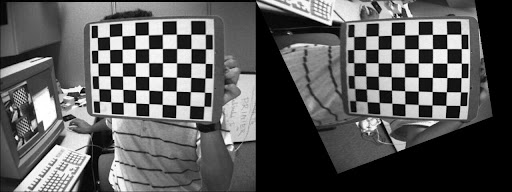
\includegraphics[width=\linewidth]{figures/homography/chessboard_marker.jpg}}
    \caption[Chessboard marker]{An example of a chessboard marker present in a scene that may be used to establish a point correspondence that would serve for a homography transformation. The rectified, fronto-parallel view demonstrates the desired effect that points present on the ``ground'' plane (in this case, the chessboard) are properly projected, whereas other points suffer from substantial distortion. \externalsrc{\cite{webhomographybasiccode}}}
    \label{fig:ChessboardMarker}
\end{figure}

\begin{figure}[t]
    \centerline{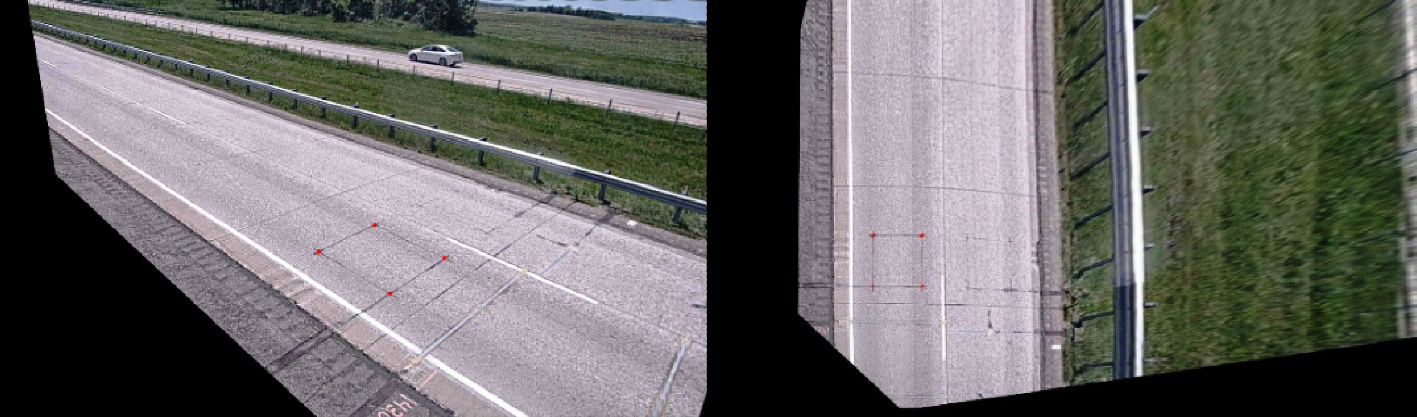
\includegraphics[width=\linewidth]{figures/homography/homography_road.png}}
    \caption[Square marker on a road]{An example of a virtual square marker present on a road that may be used to establish a point correspondence, and thus the homography transformation, too. The obtained view allows for many applications such as speed and size measurements that would otherwise be a lot more problematic in a perspectively deformed view. \externalsrc{\cite{bose2004groundplane}}}
    \label{fig:RoadMarker}
\end{figure}

A common approach to estimate the homography is to use a set of at least four $2$D point correspondences~\cite{hartley1997defense}. The points that are used for establishing the $2$D point correspondences will be referred to as keypoints. These keypoints may belong to a marker which is an object with a known shape that is either naturally occurring or artificially positioned in the scene. A regular, easy-to-detect pattern (e.g., a chessboard) is commonly utilized~\cite{zhang2016flexible} (see \figstr{}~\ref{fig:ChessboardMarker}). A single marker is identified in the image by multiple independent keypoints that have a direct correspondence to its real shape, thus making a group of point correspondences. For the sake of traffic analysis, the marker may be represented by virtually any points on the image as long as certain conditions are met (see \figstr{}~\ref{fig:RoadMarker}). However, the point correspondences established this way are often subjected to noise, thus errors may be introduced in the homography estimation. Although $4$ keypoints are satisfactory, often a greater number of keypoints is used, allowing to use optimization to minimize a suitable cost function~\cite{osuna2016multiobjective, mou2013robust}. Subsequently, an outlier removal becomes an important step in the processing pipeline, for which effective and robust algorithms such as RANSAC~\cite{fischler1981random} are usually employed.

\begin{figure}[t]
    \centerline{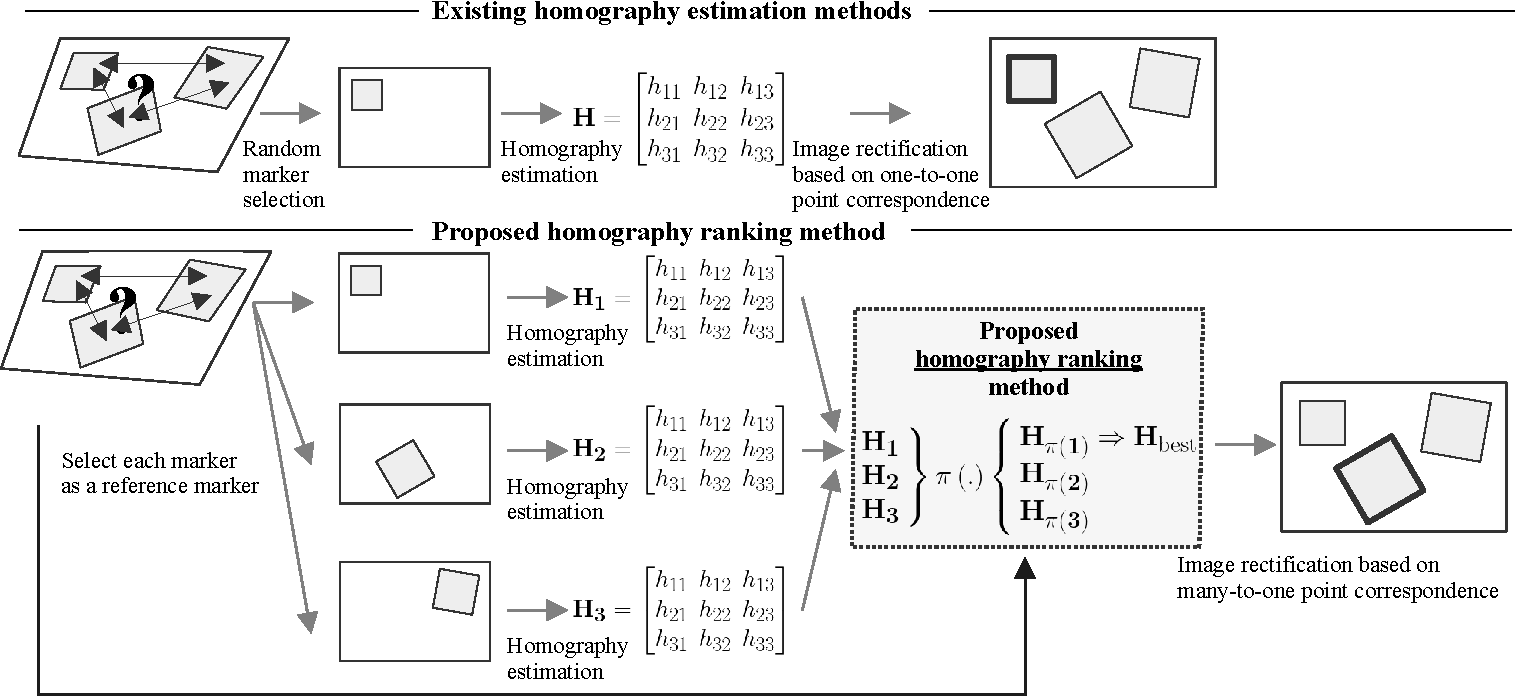
\includegraphics[width=\linewidth]{figures/homography/motivation_diagram.pdf}}
    \caption[Homography ranking motivation diagram]{A fundamental difference between existing homography estimation methods and our proposed method for homography ranking. If there are multiple markers while the information about their relative positions in the world is absent, the existing approaches can only estimate isolated homographies without the ability to select the best one. To address this issue, our method easily serves as an extension to existing approaches by exploiting multiple markers to rank the isolated homographies from the ``best'' to the ``worst''.}
    \label{fig:HomographyMotivationDiagram}
\end{figure}

A real-world application of generating a bird's-eye view over a road (see \figstr{}~\ref{fig:RoadRectification}) from a video recording when we could not use a large marker to cover a sufficient portion of the road (see \figstr{}~\ref{fig:MultipleMarkersOnRoad}) motivated this entire project. We observed that, under our conditions, the homography estimation based on a single small marker was inaccurate. Therefore, there was an attempt to utilize multiple small markers and measure their relative positions. However, as is often the case in practice, their position measurements were highly noisy at best. Thus, we had to bypass the position measurements altogether, which led us to adopt the proposed method, instead. It is crucial to emphasize that our method can also be adopted in a situation when the marker placed at various positions on the same planar surface can be seen at different frames using a static camera. Stacking the captured frames onto each other would effectively yield an artificially generated view of multiple markers.

Assume a presence of a sole marker in the scene (\figstr{}~\ref{fig:RoadMarker}). Moreover, assume the view of the marker is perspectively distorted. If we know its real shape makes at our disposal, then it is possible to compute the homography. However, when multiple copies of the same marker are visible, but their positions in the world are unknown, the detailed information about the shape is not enough to incorporate all the keypoints in the estimation. In the absence of position information, existing approaches for homography estimation based on point correspondences do not work because the projection has to preserve the proportional positions. As a result, estimating the homography while not knowing the ground-truth layout of the keypoints up to an arbitrary scale does not guarantee, and often does not even lead, to the correct result.

Under the constraints discussed above, the existing methods can only generate an isolated homography for each marker based on the one-to-one point correspondence (see \figstr{}~\ref{fig:HomographyMotivationDiagram}). Each homography may be affected by different sources of noise, e.g., low resolution, blur, or keypoint detection. Thus, the outcome of rectification may vary up to a great extent. In addition, many practical applications often use a marker that just covers a small portion of the image, so increasing susceptibility to noise as a result. The trivial solution would be to use a bigger marker that covers the majority of the estimated plane's area. But such a solution is often cumbersome. It is simply not possible to ``merge'' multiple isolated homographies together.

\begin{figure}[t]
    \centerline{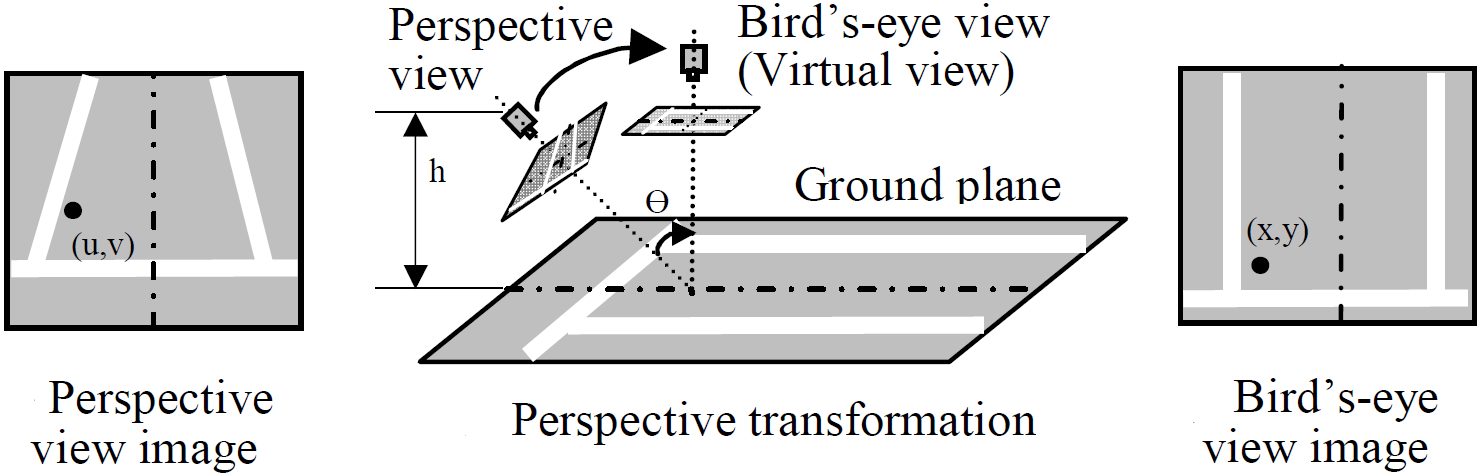
\includegraphics[width=0.8\linewidth]{figures/homography/road_rectification.png}}
    \caption[Road rectification]{A demonstration of the process of rectification when obtaining a fronto-parallel view over the road using homography. \externalsrc{\cite{luo2010low}}}
    \label{fig:RoadRectification}
\end{figure}

\begin{figure}[t]
    \centerline{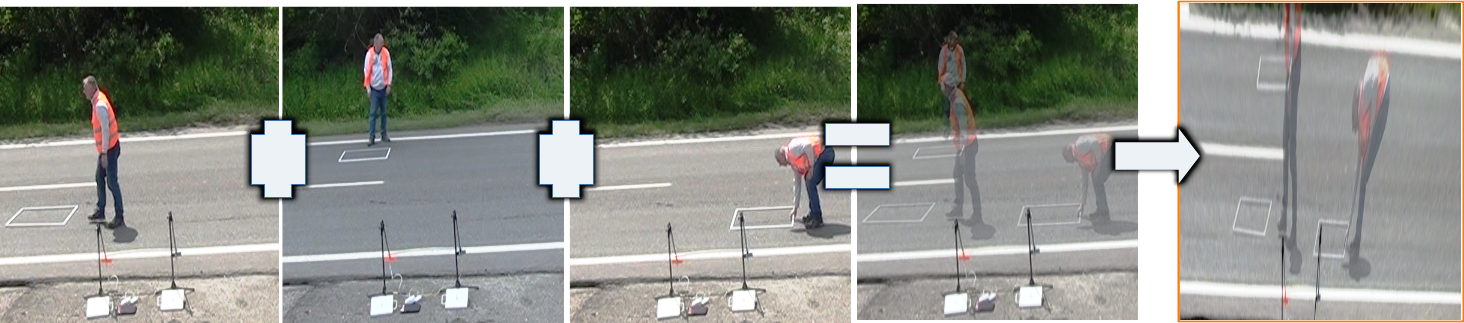
\includegraphics[width=\linewidth]{figures/homography/markers_on_the_road.png}}
    \caption[Multiple markers on the road]{A motivating real-world example for the proposed method. We can see different frames captured during a video recording that show various positions of the same marker. The picture after the ``equality'' sign is a merge of the previous frames for better illustration. Due to the use of a static camera, we may treat the positions of the given marker on individual frames as if they were captured simultaneously. However, the question remains unanswered. Given multiple markers in the absence of their position information, which one is the best to choose for rectification?}
    \label{fig:MultipleMarkersOnRoad}
\end{figure}